\documentclass[12pt, twoside]{article}
\usepackage[letterpaper, margin=1in, headsep=0.5in]{geometry}
\usepackage[english]{babel}
\usepackage[utf8]{inputenc}
\usepackage{amsmath}
\usepackage{amsfonts}
\usepackage{amssymb}
\usepackage{tikz}
\usetikzlibrary{quotes, angles}
\usepackage{graphicx}
\usepackage{enumitem}
\usepackage{multicol}

\newif\ifmeta
\metatrue %print standards and topics tags

\title{Regents Geometry}
\author{Chris Huson}
\date{September 2020}

\usepackage{fancyhdr}
\pagestyle{fancy}
\fancyhf{}
\renewcommand{\headrulewidth}{0pt} % disable the underline of the header
\raggedbottom


\fancyhead[LE]{\thepage}
\fancyhead[RO]{\thepage \\ Name: \hspace{4cm} \,\\}
\fancyhead[LO]{BECA / Dr. Huson / Geometry 07-Similarity\\* pset ID: 123}

\begin{document}

\subsubsection*{7-9DN-Analytic-proof}
\begin{enumerate}
  \subsubsection*{Proof: Using the distance formula to prove an isosceles triangle}
\item In this problem use the following theorem (copy it at the bottom of the page after your calculations): \\*[0.25cm]
    \emph{A triangle is isosceles if and only two of its sides are congruent.}\\*[0.5cm]
    Shown below is triangle $ABC$, $A(4,3)$, $B(-3,4)$, and $C(2,-1)$. \\*[0.25cm]
    Prove it is an isosceles triangle by
    \begin{enumerate}
      \item finding the length of each of the three sides,
      \item stating which sides are congruent,
      \item copying the theorem as your conclusion, adding \emph{therefore $\triangle ABC$ is isosceles}.
    \end{enumerate}
    \begin{flushright} %4 quadrant regents grid
      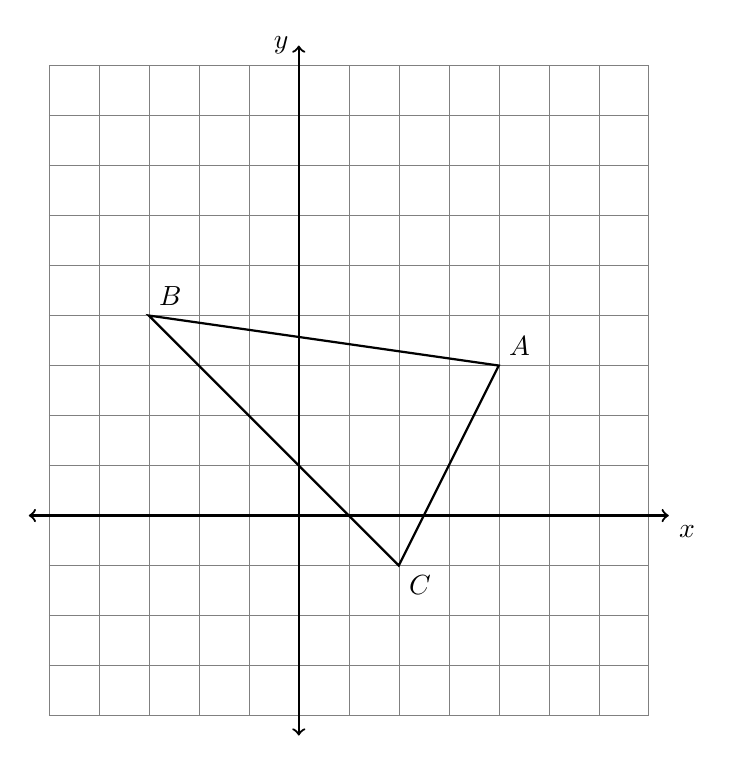
\begin{tikzpicture}[scale=.635]
        \draw [help lines] (-5,-4) grid (7,9);
        \draw [thick, <->] (-5.4,0) -- (7.4,0) node [below right] {$x$};
        \draw [thick, <->] (0,-4.4)--(0,9.4) node [left] {$y$};
        \draw [thick] (4,3) node[above right] {$A$}--
        (-3,4) node[above right] {$B$}--
        (2,-1) node[below right] {$C$}--cycle;
      \end{tikzpicture}
    \end{flushright}

\newpage
  \subsubsection*{Proof: Using slope to prove parallel sides of a trapezoid}
\item In this problem use the following theorem (copy it at the bottom of the page after your calculations): \\*[0.25cm]
  \emph{A quadrilateral is a trapezoid if and only exactly two of its sides are parallel.}\\*[0.5cm]
  David plotted $A(-1,6)$, $B(3,8)$, $C(6,-1)$, and $D(1,0)$ to form a quadrilateral. \\*[0.25cm]
  Prove that David's quadrilateral is a trapezoid by
  \begin{enumerate}
    \item finding the slope of each of the four sides,
    \item stating which opposite sides are parallel, and which opposite sides are not,
    \item copying the theorem as your conclusion, adding \emph{therefore $ABCD$ is a trapezoid}.
  \end{enumerate}
  \begin{flushright} %4 quadrant regents grid
    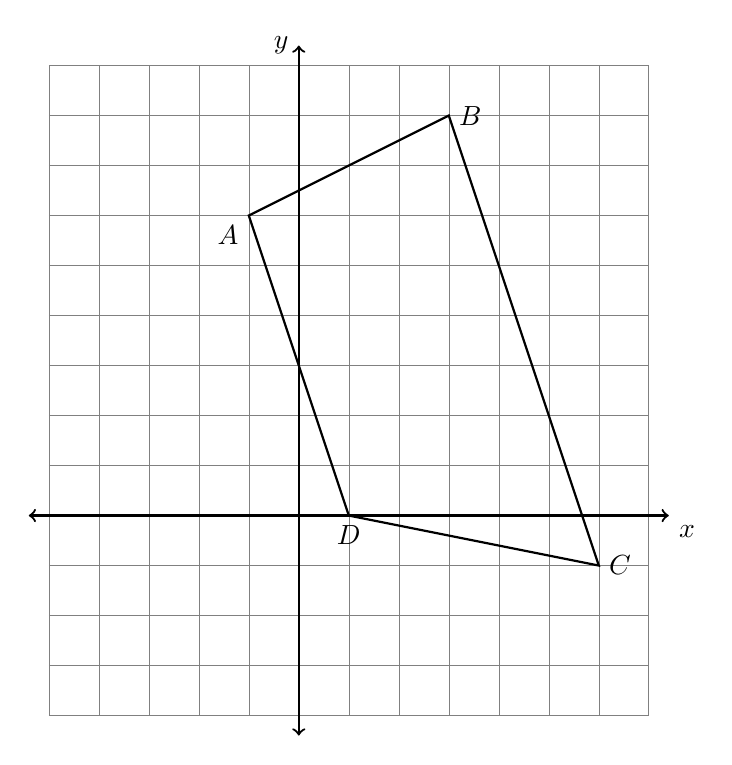
\begin{tikzpicture}[scale=.635]
      \draw [help lines] (-5,-4) grid (7,9);
      \draw [thick, <->] (-5.4,0) -- (7.4,0) node [below right] {$x$};
      \draw [thick, <->] (0,-4.4)--(0,9.4) node [left] {$y$};
      \draw [thick] (-1,6) node[below left] {$A$}--
      (3,8) node[right] {$B$}--
      (6,-1) node[right] {$C$}--
      (1,0) node[below] {$D$}--cycle;
    \end{tikzpicture}
  \end{flushright}

\end{enumerate}
\end{document}